\documentclass[aps,12pt,prd,nofootinbib,bibnotes, amsmath,amssymb,showpacs,superscriptaddress,floatfix]{revtex4-2}
\bibliographystyle{apsrev}
\usepackage[utf8]{inputenc}
\usepackage{epsf,epsfig,graphics}
\usepackage{graphicx,amsmath,mathrsfs,amssymb, amsthm,nccbbb,cancel,xcolor,wrapfig,siunitx,longtable,tabularx,CJKutf8,subfigure,float,xspace,physics,esvect,braket,enumitem,url,makeidx}
\usepackage{verbatim,color,ulem}
\usepackage{bm}
\usepackage[mathscr]{eucal}
\usepackage{hyperref}
\usepackage[toc,page]{appendix}
\usepackage[hang, flushmargin]{footmisc}
\usepackage{footnotebackref}

%%%%%%%%%%%%%%%%%%%%%%%%%%%%%%%%%%%%%%%%%%%
\begin{document}
\title{Computational Astrophysics HW3}
\author{Yi-Hsiang Kuo, 110022506}
\date{Oct. 27, 2022}
\maketitle
%\tableofcontents
%%%%%%%%%%%%%%%%%%%%%%%%%%%%%%%%%%%%%%%%%%%
\section{Exercise 2}
(1) The equation of {\bf{vector norm ($L_p$-norms)}}:
\begin{equation}
||x||_p = (\sum^n_{i = 1}|x_i|^p)^\frac{1}{p} 
\end{equation}

After calculation, we can get {\color{blue}{first and second norms $3.3$ and $2.7$ respectively}}

for {\bf{infinite norm}}, applying:
\begin{equation}
||x||_{\infty} = max|x_i|, \quad 1 \leq i \leq n
\end{equation}

and get the answer: {\color{blue}{2.6}}. \\
 
(2) For the matrix $A$, applying the {\bf{matrix norm}} formula:
\begin{equation}
||A|| = max_{x \neq 0} \frac{||Ax||}{||x||}
\end{equation}
\begin{equation}
||A||_1 = max_j \sum_{i=1}^n |a_{ij}|
\end{equation}
\begin{equation}
||A||_{\infty} = max_i \sum_{j=1}^n |a_{ij}|
\end{equation}

we can get the {\color{blue}{L1-norm (maximum absolute column sum):78}}, and the {\color{blue}{$L_{\infty}$-norm (maximum absolute row sum):83}} \\

\section{Exercise 3}
To evaluate the real root(s) of:
\begin{equation}
x^3+1.5 x^2 -5.75 x +4.37 = 0
\end{equation}

using {\color{blue}{(a) bisection method}} with initial guess from $-4.0$ to $-3.0$; {\color{blue}{(b) Newton-Raphson's method}} with initial point $x=-3.0$ and {\color{blue}{(c) secant method}} with initial guess from $-4.0$ to $-3.0$, and FIG. 1. is the comparison result.
\begin{figure}
	\centering
	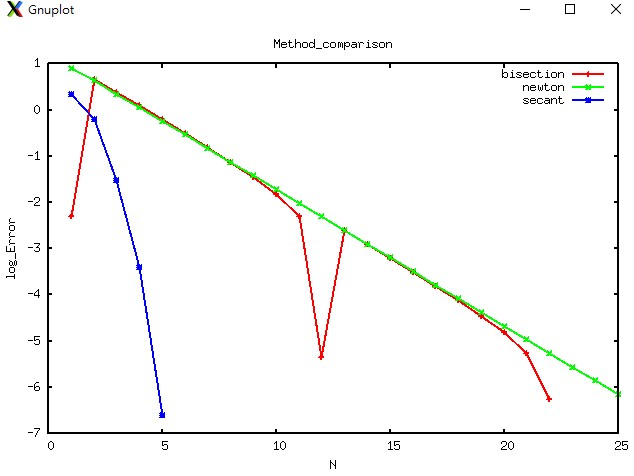
\includegraphics[width=1.0\textwidth]{EX3_Method_comparison}
	\caption{Exercise3 Method comparison}
\end{figure}

By the way, for {\color{blue}{Newton-Raphson's method}}, if our initial guess is $x=-3.5$, the iteration value N still need to approach $N=14$, it seems that {\color{blue}{(c) secant method}} is the best way here.   
    
\section{Exercise 4}
(1)(2)(3) The analytical calculations wrote on FIG. 2. : 
\begin{figure}
	\centering
	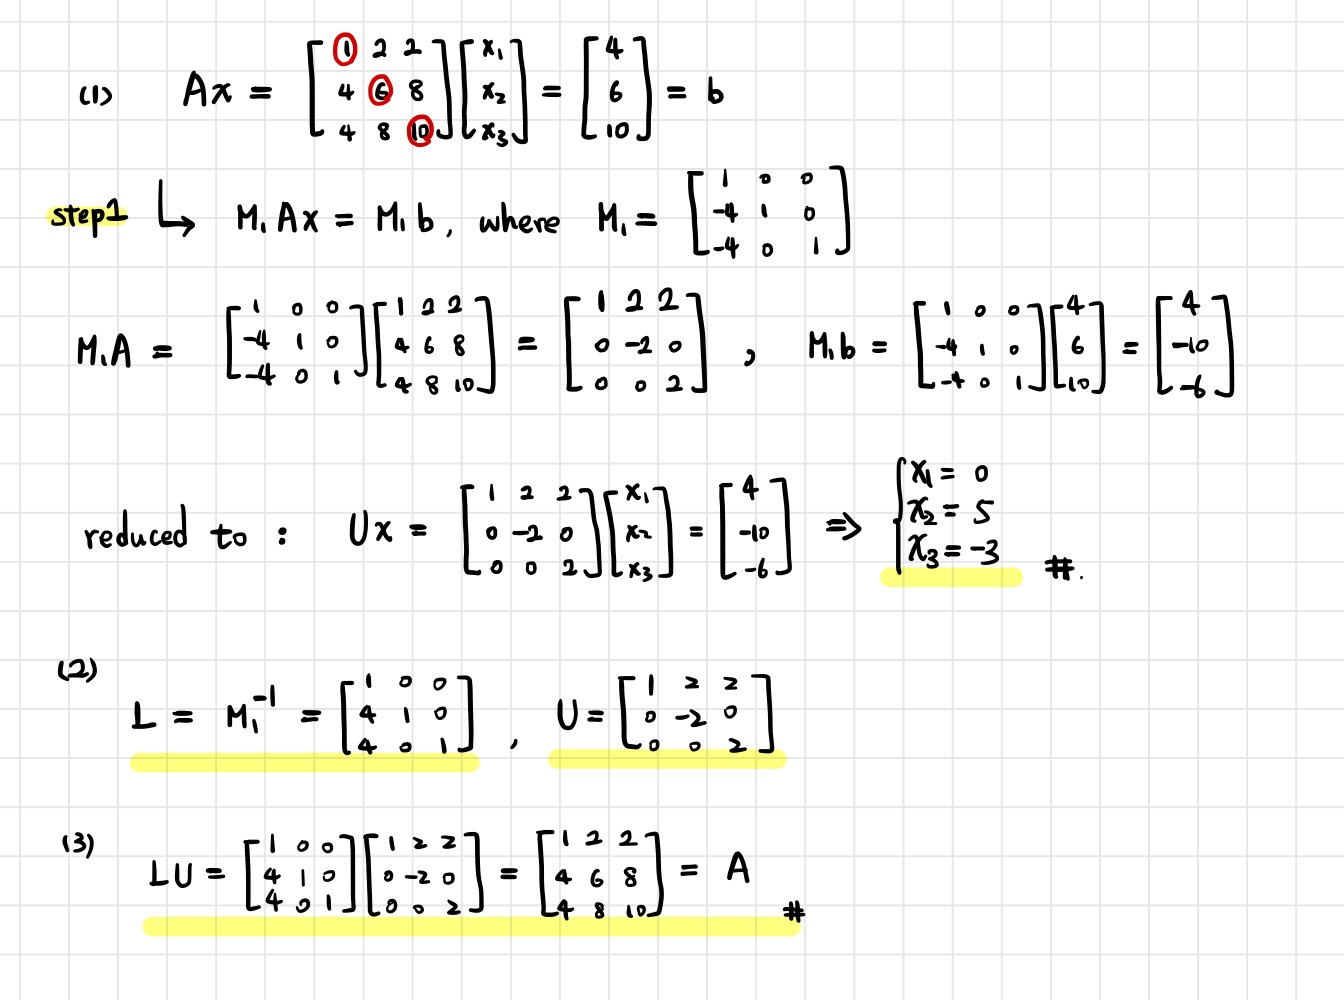
\includegraphics[width=1.0\textwidth]{EX4}
	\caption{Exercise4 Gaussian elimination}
\end{figure}



\section{Exercise 5}
(1)
To find the optimal $h$ which minimize the total error (64-bit):
\begin{equation}
\epsilon_{tot}=\epsilon_{tr}+\epsilon_{ro} \approx \frac{f^{(2)}}{2} h + \frac{\epsilon_{m}}{h}
\end{equation}

Since $f^{(2)} \approx 1$, so after differentiation we find that \textcolor{blue}{\bf{when $h \approx 4.47 \times 10^{-8}$}} \\

(2)
To find the optimal $h$ which minimize the total error of (64-bit) of {\bf{the central-difference algorithm}}:
\begin{equation}
\epsilon_{tot}=\epsilon_{tr}+\epsilon_{ro} \approx \frac{f^{(3)}}{24} h^2 + \frac{\epsilon_{m}}{h}
\end{equation}

Since $f^{(3)} \approx 1$, so after differentiation we find that \textcolor{blue}{\bf{when $h \approx 2.29 \times 10^{-5}$}} \\

(3)Put the optimal h back, we can get the minimal total error for both method, $4.47 \times 10^{-8}$ and $6.55 \times 10^{-11}$ for method 1 and method 2 respectively, {\textcolor{blue}{so method 2 is better behaved}}, also the step size $h$ is smaller for method 2.

\section{Exercise 6}
(1) I choose python to do the work and the step size $h=0.1$ for this question, and the \href{https://github.com/kuo1235/Computational-Astrophysics-2022/blob/main/astr660/Homework/HW2/Exercise6.py
}{\bf{git gub link is here}} with the result FIG. 10 and FIG. 11, however \textcolor{red}{I have not come up with the answer when $x=100$}\\ 


(2)


\bibliographystyle{apsrev}
\bibliography{Ref}
\end{document}







